%\documentclass[12pt,a4paper]{scrbook}
%\usepackage[utf8]{inputenc}
%\usepackage{amsmath}
%\usepackage{amsfonts}
%\usepackage{amssymb}
%\usepackage{graphicx}
%\usepackage{csquotes}

%\begin{document}
	
\chapter{Computer und Internet}
Hier erfährst du, welche Möglichkeiten du hast, die CIP-Pools (Computerräume) zu nutzen,  wie du Zugang zum Uni-WLAN erhältst 
und welche anderen nützlichen Dinge die Uni online anbietet.

% evtl. Infos wo/wie man sein verbleibendes Kontingent anschauen kann

\section{CIP-Pools}
In CIP-Pools\footnote{Computer-Investitions-Programm} findest du Rechnerarbeitsplätze und Drucker, teilweise auch Scanner. Das Druckerkontingent beträgt für Mathematika, Physika und Statistika 500 Seiten pro Semester. Informatika haben 600 Seiten pro Semester zur freien Verfügung. Einige CIP-Pools haben auch Farbdrucker, deren Kontingent ist kleiner (für Informatiker kostet eine Farbseite so viel wie drei schwarz-weiß Seiten).

\begin{tabularx}{\linewidth}{lX}
\textbf{Mathematik, Wirtschaftsmathematik}
& Theresienstraße 37--41, BU135 und BU136, Wendeltreppe nach unten\\
\textbf{Physik, Meteorologie}
& Schellingstraße 4 Erdgeschoss, H037 und H022\\
\textbf{Medieninformatik, Informatik}
& Oettingenstraße 67, BU102, LU112, LU114 und LU117 (Keller und Baracken)\\
\textbf{Medieninformatik zusätzlich}
& Amalienstraße 17, EG\\
\textbf{Für alle}
& Theresienstraße 37--41, 1. Stock B115 \newline
\end{tabularx}

Um in der Theresienstraße zur Anmeldemaske für dein Fach zu kommen, musst du kurz den Ausschaltknopf am Rechner hinter dem Bildschirm drücken. Informatiker und Medieninformatiker müssen die dortigen Rechner erst freischalten. Dazu gehst du auf \ref{rechnerkonfig}, meldest dich mit der Informatik-CIP-Kennung an, klickst \emph{\enquote{Change remote connection config}} $\rightarrow$ \emph{\enquote{change}} und wartest einige Minuten.

%\begin{center}
%	{
\includegraphics[width=0.6\textwidth]{comic_virus}}
%\end{center}

\begin{urlList}
	\urlItem{http://conf.cip.ifi.lmu.de/}[rechnerkonfig]
\end{urlList}

\section{Online-Dienste der LMU}
\label{sec:online}
\subsection*{Campus LMU}

Hier kannst du deine Campus-Kennung aktivieren, erhältst Zugang zum E-Mail-Account, deinem Benutzerkonto und dem Vorlesungsverzeichnis (LSF) und kannst dich von Newslettern der LMU an- und abmelden.

%\begin{itemize}
%	\item Aktivierung der Campus-Kennung
%	\item Zugang zum E-Mail-Account
%	\item Zugang zum Benutzerkonto (An-/Abmeldung von Newslettern der LMU)
%	\item Zugang zum LSF (Vorlesungsverzeichnis)
%\end{itemize}

\begin{urlList}
	\urlItem{http://www.portal.lmu.de}
\end{urlList}

\begin{center}
	{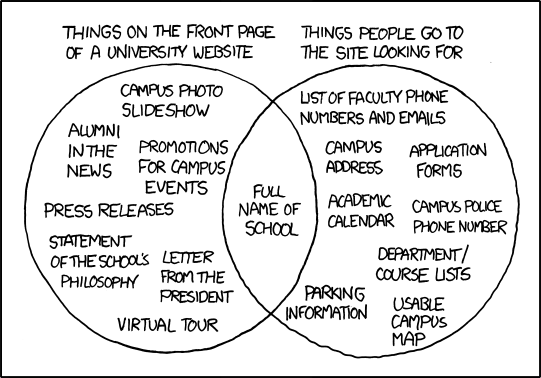
\includegraphics[width=0.6\textwidth]{comic_university}}
\end{center}

\subsection*{Online-Selbstbedienungsfunktionen}

Bescheinigungen für Immatrikulation, Studienverlauf und gezahlte Beiträge sowie das Formular zur Prüfungsanmeldung findest du hier. Diese sind online noch vor dem Versand der offiziellen Bestätigungen verfügbar, was nützlich für Arbeitsverträge ist. Außerdem kannst du deine Adressdaten und Telefonnummern ändern.

%\begin{itemize}
%	\item Bescheinigungen für Immatrikulation, Studienverlauf, gezahlte Beiträge. Diese sind online noch vor dem Versand der offiziellen Bestätigungen verfügbar (nützlich für Arbeitsverträge).
%	\item Änderung von Adressdaten und Telefonnummern
%	\item Formular zur Prüfungsanmeldung
%\end{itemize}

\begin{urlList}
	\urlItem{http://www.lmu.de/studium/studium_aktuell/neuigkeiten/studkanz/system.html}
\end{urlList}

\subsection*{Vorlesungsverzeichnis (Lehre Studium Forschung -- LSF)}

Das LSF bietet eine Übersicht über (fast) alle Veranstaltungen der LMU. Du findest hier ein, etwas merkwürdig zu bedienendes, Stundenplan-Tool, die Anmeldung zu Kursen und Klausuren (BWL, VWL) und den, in der Physik nicht immer aktuellen, Notenauszug.

%\begin{itemize}
%	\item Übersicht über (fast) alle Veranstaltungen der LMU
%	\item Stundenplan-Tool (etwas merkwürdig zu bedienen)
%	\item Anmeldung zu Kursen und Klausuren (BWL, VWL)
%	\item Notenauszug, in der Physik nicht immer aktuell
%\end{itemize}

\begin{urlList}
	\urlItem{http://www.lsf.lmu.de}
\end{urlList}


\subsection*{E-Medien}
Viele E-Books, Paper, und wissenschaftliche Journale bekannter Wissenschaftsverlage stehen LMU Mitgliedern kostenlos zur Verfügung.
Besucht man die Webseiten der entsprechenden Publikationen, fordern die Verlage einen zum Kauf auf.
Besucht man die Webseite jedoch über den E-Medien-Login der Universitätsbibliothek \ref{emedien} stehen einem die Werke kostenlos zum Download bereit.
\begin{urlList}
	\urlItem{http://emedien.ub.uni-muenchen.de/}[emedien]
\end{urlList}

\subsection*{Microsoft DreamSpark \subjectList{\subjectI{}\subjectMI{}\subjectP{}}}
Studika der Physik und Informatik (auch im Nebenfach) bekommen über
Microsoft DreamSpark (früher MSDNAA) viele Microsoftproduktlizenzen
gratis, darunter Windows, Visual Studio und viele
Microsoft Office-Komponenten, jedoch \textbf{nicht} Word, Excel und PowerPoint.

\begin{urlList}
	\urlItem{http://tools.rz.ifi.lmu.de/cipconf/index.rb?op=msdnaa}
	\urlItem{https://msdnaa.physik.uni-muenchen.de/}
\end{urlList}

\subsection*{UniWorX\subjectList{\subjectI{}\subjectMI{}}}

Informatiker und Medieninformatiker können sich hier zu Kursen und Klausuren anmelden, ihre Noten und die Statistiken zu den Klausuren einsehen sowie Übungsblätter abgeben. UniWorx ist mit der Campus- oder CIP-Kennung nutzbar.

%\begin{itemize}
%	\item Anmeldung zu Kursen und Klausuren
%	\item Einsicht deiner Noten und Statistiken zu deinen Klausuren
%	\item Abgabe von Übungsblättern
%	\item Mit Campus- oder CIP-Kennung nutzbar
%\end{itemize}

\begin{urlList}
	\urlItem{http://www.uniworx.ifi.lmu.de}
\end{urlList}

\subsection*{Prüfungsverwaltungs- und Informationssystem (PVI)\subjectList{\subjectI{}\subjectMI{}}}

Im PVI findest du deinen Notenauszug und die verbuchten Prüfungen.

%\begin{itemize}
%	\item Notenauszug, verbuchte Prüfungen
%\end{itemize}

\begin{urlList}
	\urlItem{http://pvineu.ifi.lmu.de}
\end{urlList}


\section{E-Mail}
Damit du nicht unterfordert wirst, besitzt du direkt von Anfang an mindestens zwei verschiedene E-Mail-Adressen. Bei beiden E-Mail-Adressen ist es möglich und auch wärmstens empfohlen eine Weiterleitung einzurichten.

Die Campus-Adresse besitzt jedes Studikon der LMU, während die CIP-Adresse für die Nutzer der CIP-Pools ist.

\subsection*{Für alle Studika der LMU}
\begin{itemize}
	\item[]<vorname.nachname>@campus.lmu.de (bzw. was ihr angegeben habt)
\end{itemize}
Zum Weiterleiten einfach unter \ref{webmail} links unten auf Weiterleitung klicken und eine andere E-Mail-Adresse angeben.

\begin{urlList}
	\urlItem{https://mailbox.portal.uni-muenchen.de}[webmail]
\end{urlList}

\subsection*{Mathematik und Wirtschaftsmathematik\subjectList{\subjectM\subjectW}}
\begin{itemize}
	\item[]<seltsameKombination>@math.lmu.de
\end{itemize}
Deinen Account kannst du bei Herrn Spann (Theresienstraße 37--41, B124) beantragen. Die Weiterleitung erfolgt über das Shell-Kommando \verb|echo "neue Adresse" >~/.forward|. 

\subsection*{Informatik und Medieninformatik \subjectList{\subjectI\subjectMI}}
\begin{itemize}
	\item[]<accountname>@cip.ifi.lmu.de
\end{itemize}
Sollte unbedingt abgerufen oder weitergeleitet werden, da hierüber der Großteil des Informatik-Mailverkehrs abläuft. Das Passwort wird während der Anmeldung vergeben, die Kennung kannst du während der O"~Phase, in den ersten zwei Wochen des Semesters zu Blockterminen oder nach dem 15.\ Oktober zu den Sprechstunden der RBG\footnote{Rechnerbetriebsgruppe} 
(Mo--Do, 14--17 Uhr) jeweils in der Oettingenstraße 67, in LU113. beantragen-

\begin{urlList}
		\urlItem{https://webmail.ifi.lmu.de}
		\urlItem{http://www.rz.ifi.lmu.de/Dienste/Mailsystem.html}
\end{urlList}

\subsection*{Physik und Meteorologie\subjectList{\subjectP}}
\begin{itemize}
	\item[]<vorname.nachname>@physik.uni-muenchen.de
\end{itemize}
An diese Adresse werden Ankündigungen des Prüfungsamtes und Physik-Newsletter gesendet.
Das Passwort ist dasselbe wie für die Campus-Adresse.

\begin{urlList}
	\urlItem{http://webmail.physik.uni-muenchen.de}
	\urlItem{http://www.it.physik.uni-muenchen.de/dienste/kommunikation/e-mail}
\end{urlList}

\section{IRC}
IRC ist ein steinaltes, minimalistisches und nicht totzukriegendes
Chatprotokoll für Dinge, die nicht ganz eine E-Mail wert sind. Während die Uni
es nicht offiziell nutzt, ist es beliebt unter Studenten, speziell unter
Informatikern und uns Fachschaftlern. Manch einer zieht es sogar Facebook vor!

Das IRC ist aufgeteilt in Kanäle, die auf Netzwerken leben. Um dich zu einem
Netzwerk zu verbinden, brauchst du meist einen Client, aber viele Netzwerke
bieten für Anfänger auch Webchats an. Uns findest du im Kanal \#gaf auf dem
Netzwerk freenode.

\begin{urlList}
	\urlItem{http://www.irchelp.org/irchelp/clients/}
	\urlItem{https://webchat.freenode.net/}
\end{urlList}



\section{Internet / WLAN}
Um mit deinem Laptop in der Uni ins Internet zu gehen, brauchst du
deine Campus-Kennung. Damit lassen sich die WLAN-Services des
Leibniz-Rechen\-zentrums (LRZ) nutzen.

\subsection*{Eduroam}
Wir empfehlen dir, das WLAN mit dem Namen (SSID) \emph{eduroam}, auf deinen Geräten einzurichten. Mit diesem einmal eingerichteten Eduroam kannst du weltweit an vielen Universitäten und Forschungsinstituten automatisch das dortige WLAN nutzen. Unter \ref{eduroam} findest du ausführliche Anleitungen für die meisten Betriebssysteme und Smart\-phones 
(die benötigte LRZ-Kennung findest du in deinem Campus-Account unter \enquote{Benutzerkonto} $\rightarrow$ \enquote{E-Mail-Einstellungen}).

%TODO noch ein Hinweis auf das weniger gefüllte eduroam-a?
Falls du nun in der Uni sitzt und dich fragst, wie du ohne Internet
die Anleitung durchlesen oder deine LRZ-Kennung herausfinden sollst, 
findest du die Antwort im Abschnitt LRZ.
\begin{urlList}
	\urlItem{http://www.lrz.de/services/netz/mobil/eduroam}[eduroam]
\end{urlList}

\subsection*{LRZ}
Außer Eduroam gibt es noch die Möglichkeit, das Netz mit der SSID
\emph{lrz} zu verwenden. \emph{lrz} ist zunächst ein unverschlüsseltes
Netzwerk, das nur den Zugriff auf die Website des
Leibniz-Rechen\-zentrums gestattet. Hier kannst du dir entweder die 
Anleitung für \mbox{\emph{eduroam}} durchlesen, oder die
vorkonfigurierte Clientsoftware AnyConnect herunterladen, welche dich
durch Anmeldung mit deiner Campuskennung in ein VPN (Virtual Private
Network) des LRZ einbucht. Aus Netzwerksicht verhält sich dein Rechner
dann wie alle anderen Rechner im MWN (Münchner Wissenschaftsnetz). So
kannst du nicht nur normal surfen, sondern auch von außen auf das
MWN zugreifen um zum Beispiel bestimmte Artikel aus der Bibliothek zu lesen.

Die Clientsoftware ist übrigens außerhalb der Uni praktisch, um deine
HTTP"=Verbindungen zu verschlüsseln, etwa wenn du dich in einem
ungeschützen WLAN befindest.

%\end{document}
